% Options for packages loaded elsewhere
\PassOptionsToPackage{unicode}{hyperref}
\PassOptionsToPackage{hyphens}{url}
%
\documentclass[
]{article}
\usepackage{amsmath,amssymb}
\usepackage{iftex}
\ifPDFTeX
  \usepackage[T1]{fontenc}
  \usepackage[utf8]{inputenc}
  \usepackage{textcomp} % provide euro and other symbols
\else % if luatex or xetex
  \usepackage{unicode-math} % this also loads fontspec
  \defaultfontfeatures{Scale=MatchLowercase}
  \defaultfontfeatures[\rmfamily]{Ligatures=TeX,Scale=1}
\fi
\usepackage{lmodern}
\ifPDFTeX\else
  % xetex/luatex font selection
\fi
% Use upquote if available, for straight quotes in verbatim environments
\IfFileExists{upquote.sty}{\usepackage{upquote}}{}
\IfFileExists{microtype.sty}{% use microtype if available
  \usepackage[]{microtype}
  \UseMicrotypeSet[protrusion]{basicmath} % disable protrusion for tt fonts
}{}
\makeatletter
\@ifundefined{KOMAClassName}{% if non-KOMA class
  \IfFileExists{parskip.sty}{%
    \usepackage{parskip}
  }{% else
    \setlength{\parindent}{0pt}
    \setlength{\parskip}{6pt plus 2pt minus 1pt}}
}{% if KOMA class
  \KOMAoptions{parskip=half}}
\makeatother
\usepackage{xcolor}
\usepackage[margin=1in]{geometry}
\usepackage{color}
\usepackage{fancyvrb}
\newcommand{\VerbBar}{|}
\newcommand{\VERB}{\Verb[commandchars=\\\{\}]}
\DefineVerbatimEnvironment{Highlighting}{Verbatim}{commandchars=\\\{\}}
% Add ',fontsize=\small' for more characters per line
\usepackage{framed}
\definecolor{shadecolor}{RGB}{248,248,248}
\newenvironment{Shaded}{\begin{snugshade}}{\end{snugshade}}
\newcommand{\AlertTok}[1]{\textcolor[rgb]{0.94,0.16,0.16}{#1}}
\newcommand{\AnnotationTok}[1]{\textcolor[rgb]{0.56,0.35,0.01}{\textbf{\textit{#1}}}}
\newcommand{\AttributeTok}[1]{\textcolor[rgb]{0.13,0.29,0.53}{#1}}
\newcommand{\BaseNTok}[1]{\textcolor[rgb]{0.00,0.00,0.81}{#1}}
\newcommand{\BuiltInTok}[1]{#1}
\newcommand{\CharTok}[1]{\textcolor[rgb]{0.31,0.60,0.02}{#1}}
\newcommand{\CommentTok}[1]{\textcolor[rgb]{0.56,0.35,0.01}{\textit{#1}}}
\newcommand{\CommentVarTok}[1]{\textcolor[rgb]{0.56,0.35,0.01}{\textbf{\textit{#1}}}}
\newcommand{\ConstantTok}[1]{\textcolor[rgb]{0.56,0.35,0.01}{#1}}
\newcommand{\ControlFlowTok}[1]{\textcolor[rgb]{0.13,0.29,0.53}{\textbf{#1}}}
\newcommand{\DataTypeTok}[1]{\textcolor[rgb]{0.13,0.29,0.53}{#1}}
\newcommand{\DecValTok}[1]{\textcolor[rgb]{0.00,0.00,0.81}{#1}}
\newcommand{\DocumentationTok}[1]{\textcolor[rgb]{0.56,0.35,0.01}{\textbf{\textit{#1}}}}
\newcommand{\ErrorTok}[1]{\textcolor[rgb]{0.64,0.00,0.00}{\textbf{#1}}}
\newcommand{\ExtensionTok}[1]{#1}
\newcommand{\FloatTok}[1]{\textcolor[rgb]{0.00,0.00,0.81}{#1}}
\newcommand{\FunctionTok}[1]{\textcolor[rgb]{0.13,0.29,0.53}{\textbf{#1}}}
\newcommand{\ImportTok}[1]{#1}
\newcommand{\InformationTok}[1]{\textcolor[rgb]{0.56,0.35,0.01}{\textbf{\textit{#1}}}}
\newcommand{\KeywordTok}[1]{\textcolor[rgb]{0.13,0.29,0.53}{\textbf{#1}}}
\newcommand{\NormalTok}[1]{#1}
\newcommand{\OperatorTok}[1]{\textcolor[rgb]{0.81,0.36,0.00}{\textbf{#1}}}
\newcommand{\OtherTok}[1]{\textcolor[rgb]{0.56,0.35,0.01}{#1}}
\newcommand{\PreprocessorTok}[1]{\textcolor[rgb]{0.56,0.35,0.01}{\textit{#1}}}
\newcommand{\RegionMarkerTok}[1]{#1}
\newcommand{\SpecialCharTok}[1]{\textcolor[rgb]{0.81,0.36,0.00}{\textbf{#1}}}
\newcommand{\SpecialStringTok}[1]{\textcolor[rgb]{0.31,0.60,0.02}{#1}}
\newcommand{\StringTok}[1]{\textcolor[rgb]{0.31,0.60,0.02}{#1}}
\newcommand{\VariableTok}[1]{\textcolor[rgb]{0.00,0.00,0.00}{#1}}
\newcommand{\VerbatimStringTok}[1]{\textcolor[rgb]{0.31,0.60,0.02}{#1}}
\newcommand{\WarningTok}[1]{\textcolor[rgb]{0.56,0.35,0.01}{\textbf{\textit{#1}}}}
\usepackage{longtable,booktabs,array}
\usepackage{calc} % for calculating minipage widths
% Correct order of tables after \paragraph or \subparagraph
\usepackage{etoolbox}
\makeatletter
\patchcmd\longtable{\par}{\if@noskipsec\mbox{}\fi\par}{}{}
\makeatother
% Allow footnotes in longtable head/foot
\IfFileExists{footnotehyper.sty}{\usepackage{footnotehyper}}{\usepackage{footnote}}
\makesavenoteenv{longtable}
\usepackage{graphicx}
\makeatletter
\def\maxwidth{\ifdim\Gin@nat@width>\linewidth\linewidth\else\Gin@nat@width\fi}
\def\maxheight{\ifdim\Gin@nat@height>\textheight\textheight\else\Gin@nat@height\fi}
\makeatother
% Scale images if necessary, so that they will not overflow the page
% margins by default, and it is still possible to overwrite the defaults
% using explicit options in \includegraphics[width, height, ...]{}
\setkeys{Gin}{width=\maxwidth,height=\maxheight,keepaspectratio}
% Set default figure placement to htbp
\makeatletter
\def\fps@figure{htbp}
\makeatother
\setlength{\emergencystretch}{3em} % prevent overfull lines
\providecommand{\tightlist}{%
  \setlength{\itemsep}{0pt}\setlength{\parskip}{0pt}}
\setcounter{secnumdepth}{-\maxdimen} % remove section numbering
\usepackage{booktabs}
\usepackage{longtable}
\usepackage{array}
\usepackage{multirow}
\usepackage{wrapfig}
\usepackage{float}
\usepackage{colortbl}
\usepackage{pdflscape}
\usepackage{tabu}
\usepackage{threeparttable}
\usepackage{threeparttablex}
\usepackage[normalem]{ulem}
\usepackage{makecell}
\usepackage{xcolor}
\ifLuaTeX
  \usepackage{selnolig}  % disable illegal ligatures
\fi
\usepackage{bookmark}
\IfFileExists{xurl.sty}{\usepackage{xurl}}{} % add URL line breaks if available
\urlstyle{same}
\hypersetup{
  pdftitle={Business Case: Target SQL},
  pdfauthor={Shayantan Dey},
  hidelinks,
  pdfcreator={LaTeX via pandoc}}

\title{Business Case: Target SQL}
\usepackage{etoolbox}
\makeatletter
\providecommand{\subtitle}[1]{% add subtitle to \maketitle
  \apptocmd{\@title}{\par {\large #1 \par}}{}{}
}
\makeatother
\subtitle{Scaler DS ML}
\author{Shayantan Dey}
\date{Sat 20th July}

\begin{document}
\maketitle

\subsubsection{Context:}\label{context}

Target is a globally renowned brand and a prominent retailer in the
United States. Target makes itself a preferred shopping destination by
offering outstanding value, inspiration, innovation and an exceptional
guest experience that no other retailer can deliver.

This particular business case focuses on the operations of Target in
Brazil and provides insightful information about 100,000 orders placed
between 2016 and 2018. The dataset offers a comprehensive view of
various dimensions including the order status, price, payment and
freight performance, customer location, product attributes, and customer
reviews.

By analyzing this extensive dataset, it becomes possible to gain
valuable insights into Target's operations in Brazil. The information
can shed light on various aspects of the business, such as order
processing, pricing strategies, payment and shipping efficiency,
customer demographics, product characteristics, and customer
satisfaction levels.

\subsubsection{Dataset:}\label{dataset}

The data is available in 8 csv files at
\href{https://drive.google.com/drive/folders/1TGEc66YKbD443nslRi1bWgVd238gJCnb}{Google
Drive}

\begin{enumerate}
\def\labelenumi{\arabic{enumi}.}
\tightlist
\item
  customers.csv\\
\item
  sellers.csv\\
\item
  order\_items.csv\\
\item
  geolocation.csv\\
\item
  payments.csv\\
\item
  reviews.csv\\
\item
  orders.csv\\
\item
  products.csv
\end{enumerate}

The column description for these csv files is given below.

The \textbf{customers.csv} contain following features:

\begin{longtable}[]{@{}ll@{}}
\toprule\noalign{}
Code & Name \\
\midrule\noalign{}
\endhead
\bottomrule\noalign{}
\endlastfoot
\texttt{dnorm(x,\ mean,\ sd)} & probability density function \\
\texttt{pnorm(q,\ mean,\ sd)} & cumulative distribution function \\
\texttt{qnorm(p,\ mean,\ sd)} & quantile function \\
\texttt{rnorm(n,\ mean,\ sd)} & random number generator \\
\end{longtable}

The \textbf{sellers.csv} contains following features:

\begin{longtable}[]{@{}ll@{}}
\toprule\noalign{}
Code & Name \\
\midrule\noalign{}
\endhead
\bottomrule\noalign{}
\endlastfoot
\texttt{dnorm(x,\ mean,\ sd)} & probability density function \\
\texttt{pnorm(q,\ mean,\ sd)} & cumulative distribution function \\
\texttt{qnorm(p,\ mean,\ sd)} & quantile function \\
\texttt{rnorm(n,\ mean,\ sd)} & random number generator \\
\end{longtable}

\subsubsection{Dataset schema:}\label{dataset-schema}

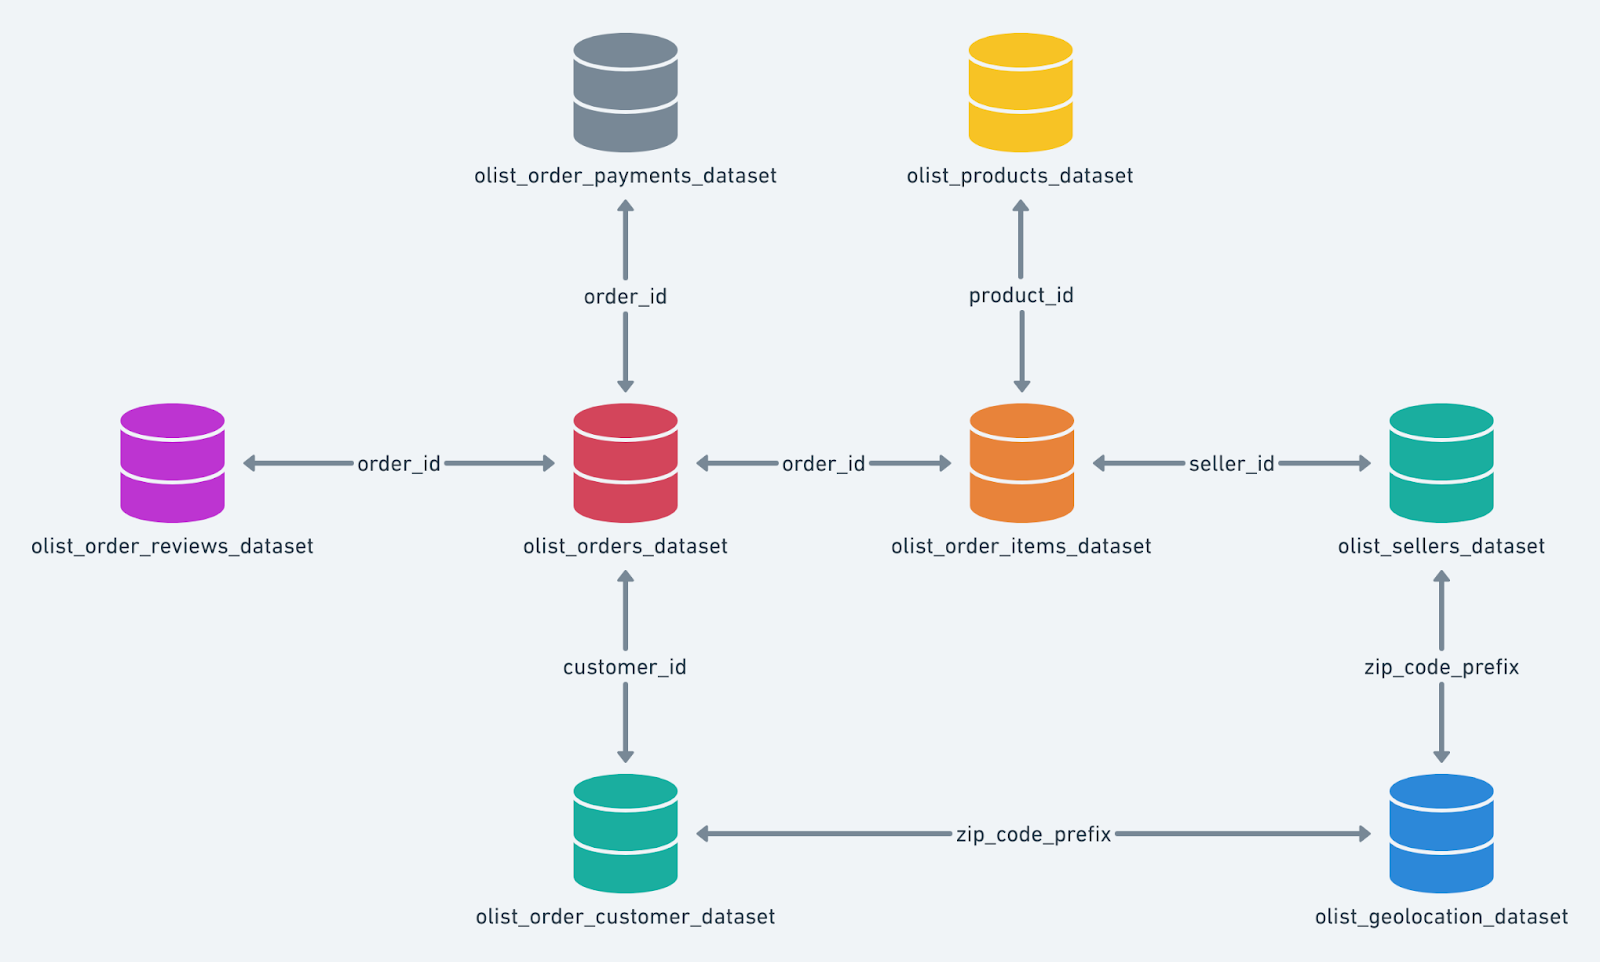
\includegraphics{dbDiag.png}

\subsubsection{Problem Statement:}\label{problem-statement}

Assuming you are a data analyst/ scientist at Target, you have been
assigned the task of analyzing the given dataset to extract valuable
insights and provide actionable recommendations.

\textbf{What does `good' look like?}

\textbf{1. Import the dataset and do usual exploratory analysis steps
like checking the structure \& characteristics of the dataset:}

1.1. Data type of all columns in the ``customers'' table.

\begin{Shaded}
\begin{Highlighting}[]
\NormalTok{PRAGMA table\_info(customers);}
\end{Highlighting}
\end{Shaded}

\begin{longtable}[]{@{}lllrlr@{}}
\caption{5 records}\tabularnewline
\toprule\noalign{}
cid & name & type & notnull & dflt\_value & pk \\
\midrule\noalign{}
\endfirsthead
\toprule\noalign{}
cid & name & type & notnull & dflt\_value & pk \\
\midrule\noalign{}
\endhead
\bottomrule\noalign{}
\endlastfoot
0 & customer\_id & TEXT & 0 & NA & 0 \\
1 & customer\_unique\_id & TEXT & 0 & NA & 0 \\
2 & customer\_zip\_code\_prefix & INTEGER & 0 & NA & 0 \\
3 & customer\_city & TEXT & 0 & NA & 0 \\
4 & customer\_state & TEXT & 0 & NA & 0 \\
\end{longtable}

1.2. Get the time range between which the orders were placed.

\begin{Shaded}
\begin{Highlighting}[]
\KeywordTok{SELECT} 
    \FunctionTok{MIN}\NormalTok{(order\_purchase\_timestamp) }\KeywordTok{AS}\NormalTok{ order\_start\_date, }
    \FunctionTok{MAX}\NormalTok{(order\_purchase\_timestamp) }\KeywordTok{AS}\NormalTok{ order\_end\_date,}
    \FunctionTok{ROUND}\NormalTok{((julianday(}\FunctionTok{MAX}\NormalTok{(order\_purchase\_timestamp)) }\OperatorTok{{-}} 
\NormalTok{      julianday(}\FunctionTok{MIN}\NormalTok{(order\_purchase\_timestamp))), }\DecValTok{2}\NormalTok{) }\KeywordTok{AS}\NormalTok{ order\_time\_range\_days}
\KeywordTok{FROM} 
\NormalTok{    orders;}
\end{Highlighting}
\end{Shaded}

\begin{longtable}[]{@{}llr@{}}
\caption{1 records}\tabularnewline
\toprule\noalign{}
order\_start\_date & order\_end\_date & order\_time\_range\_days \\
\midrule\noalign{}
\endfirsthead
\toprule\noalign{}
order\_start\_date & order\_end\_date & order\_time\_range\_days \\
\midrule\noalign{}
\endhead
\bottomrule\noalign{}
\endlastfoot
2016-09-04 21:15:19 & 2018-10-17 17:30:18 & 772.84 \\
\end{longtable}

1.3. Count the Cities \& States of customers who ordered during the
given period.

\begin{Shaded}
\begin{Highlighting}[]
\KeywordTok{SELECT} \OperatorTok{*} \KeywordTok{FROM}\NormalTok{ orders }\KeywordTok{LIMIT} \DecValTok{10}\NormalTok{;}
\end{Highlighting}
\end{Shaded}

\begin{longtable}[]{@{}
  >{\raggedright\arraybackslash}p{(\columnwidth - 14\tabcolsep) * \real{0.1549}}
  >{\raggedright\arraybackslash}p{(\columnwidth - 14\tabcolsep) * \real{0.1549}}
  >{\raggedright\arraybackslash}p{(\columnwidth - 14\tabcolsep) * \real{0.0610}}
  >{\raggedright\arraybackslash}p{(\columnwidth - 14\tabcolsep) * \real{0.1174}}
  >{\raggedright\arraybackslash}p{(\columnwidth - 14\tabcolsep) * \real{0.0939}}
  >{\raggedright\arraybackslash}p{(\columnwidth - 14\tabcolsep) * \real{0.1362}}
  >{\raggedright\arraybackslash}p{(\columnwidth - 14\tabcolsep) * \real{0.1408}}
  >{\raggedright\arraybackslash}p{(\columnwidth - 14\tabcolsep) * \real{0.1408}}@{}}
\caption{Displaying records 1 - 10}\tabularnewline
\toprule\noalign{}
\begin{minipage}[b]{\linewidth}\raggedright
order\_id
\end{minipage} & \begin{minipage}[b]{\linewidth}\raggedright
customer\_id
\end{minipage} & \begin{minipage}[b]{\linewidth}\raggedright
order\_status
\end{minipage} & \begin{minipage}[b]{\linewidth}\raggedright
order\_purchase\_timestamp
\end{minipage} & \begin{minipage}[b]{\linewidth}\raggedright
order\_approved\_at
\end{minipage} & \begin{minipage}[b]{\linewidth}\raggedright
order\_delivered\_carrier\_date
\end{minipage} & \begin{minipage}[b]{\linewidth}\raggedright
order\_delivered\_customer\_date
\end{minipage} & \begin{minipage}[b]{\linewidth}\raggedright
order\_estimated\_delivery\_date
\end{minipage} \\
\midrule\noalign{}
\endfirsthead
\toprule\noalign{}
\begin{minipage}[b]{\linewidth}\raggedright
order\_id
\end{minipage} & \begin{minipage}[b]{\linewidth}\raggedright
customer\_id
\end{minipage} & \begin{minipage}[b]{\linewidth}\raggedright
order\_status
\end{minipage} & \begin{minipage}[b]{\linewidth}\raggedright
order\_purchase\_timestamp
\end{minipage} & \begin{minipage}[b]{\linewidth}\raggedright
order\_approved\_at
\end{minipage} & \begin{minipage}[b]{\linewidth}\raggedright
order\_delivered\_carrier\_date
\end{minipage} & \begin{minipage}[b]{\linewidth}\raggedright
order\_delivered\_customer\_date
\end{minipage} & \begin{minipage}[b]{\linewidth}\raggedright
order\_estimated\_delivery\_date
\end{minipage} \\
\midrule\noalign{}
\endhead
\bottomrule\noalign{}
\endlastfoot
e481f51cbdc54678b7cc49136f2d6af7 & 9ef432eb6251297304e76186b10a928d &
delivered & 2017-10-02 10:56:33 & 2017-10-02 11:07:15 & 2017-10-04
19:55:00 & 2017-10-10 21:25:13 & 2017-10-18 00:00:00 \\
53cdb2fc8bc7dce0b6741e2150273451 & b0830fb4747a6c6d20dea0b8c802d7ef &
delivered & 2018-07-24 20:41:37 & 2018-07-26 03:24:27 & 2018-07-26
14:31:00 & 2018-08-07 15:27:45 & 2018-08-13 00:00:00 \\
47770eb9100c2d0c44946d9cf07ec65d & 41ce2a54c0b03bf3443c3d931a367089 &
delivered & 2018-08-08 08:38:49 & 2018-08-08 08:55:23 & 2018-08-08
13:50:00 & 2018-08-17 18:06:29 & 2018-09-04 00:00:00 \\
949d5b44dbf5de918fe9c16f97b45f8a & f88197465ea7920adcdbec7375364d82 &
delivered & 2017-11-18 19:28:06 & 2017-11-18 19:45:59 & 2017-11-22
13:39:59 & 2017-12-02 00:28:42 & 2017-12-15 00:00:00 \\
ad21c59c0840e6cb83a9ceb5573f8159 & 8ab97904e6daea8866dbdbc4fb7aad2c &
delivered & 2018-02-13 21:18:39 & 2018-02-13 22:20:29 & 2018-02-14
19:46:34 & 2018-02-16 18:17:02 & 2018-02-26 00:00:00 \\
a4591c265e18cb1dcee52889e2d8acc3 & 503740e9ca751ccdda7ba28e9ab8f608 &
delivered & 2017-07-09 21:57:05 & 2017-07-09 22:10:13 & 2017-07-11
14:58:04 & 2017-07-26 10:57:55 & 2017-08-01 00:00:00 \\
136cce7faa42fdb2cefd53fdc79a6098 & ed0271e0b7da060a393796590e7b737a &
invoiced & 2017-04-11 12:22:08 & 2017-04-13 13:25:17 & & & 2017-05-09
00:00:00 \\
6514b8ad8028c9f2cc2374ded245783f & 9bdf08b4b3b52b5526ff42d37d47f222 &
delivered & 2017-05-16 13:10:30 & 2017-05-16 13:22:11 & 2017-05-22
10:07:46 & 2017-05-26 12:55:51 & 2017-06-07 00:00:00 \\
76c6e866289321a7c93b82b54852dc33 & f54a9f0e6b351c431402b8461ea51999 &
delivered & 2017-01-23 18:29:09 & 2017-01-25 02:50:47 & 2017-01-26
14:16:31 & 2017-02-02 14:08:10 & 2017-03-06 00:00:00 \\
e69bfb5eb88e0ed6a785585b27e16dbf & 31ad1d1b63eb9962463f764d4e6e0c9d &
delivered & 2017-07-29 11:55:02 & 2017-07-29 12:05:32 & 2017-08-10
19:45:24 & 2017-08-16 17:14:30 & 2017-08-23 00:00:00 \\
\end{longtable}

\end{document}
